\documentclass[journal,12pt,twocolumn]{IEEEtran}
\usepackage{cite}
\usepackage{amsmath,amssymb,amsfonts,amsthm}
\usepackage{graphicx}

% Title and author information
\title{NCERT DISCRETE 10.5.4 Q1}
\author{EE23BTECH11214 - Harsha Vardhan Kumar}

\begin{document}
\maketitle

% Problem statement
\noindent \textbf{Question}:
Which term of the AP: 121, 117, 113, \ldots, is its first negative term?

% Solution
\textbf{Solution}:
\begin{table}[htbp]
\centering
\begin{tabular}{|l|l|c|}
\hline
\textbf{Symbol} & \textbf{Description} & \textbf{Value} \\
\hline
$x\sbrak{n}$ & General term & \(121 - 4n\) \\
\hline
$x\sbrak{z}$ & Initial term & 121 \\
\hline
$d$ & Common difference & 4 \\
\hline
\end{tabular}

\caption{parameters list}
\end{table}

\begin{align}
x[n] &= 121 - 4n < 0 \\
n &> \frac{121}{4} 
\end{align}
The first negative term in the sequence occurs at 
\[ n = 31 \]
Z-transform of this sequence:
\begin{align}
X(z) &= \sum_{n=0}^{\infty} x[n]z^{-n} \\
&= \sum_{n=0}^{\infty} (121 - 4n)z^{-n}
\end{align}
\begin{align}
    X(z) &= \frac{z(121z - 125)}{(z - 1)^2} \quad \abs{z}>\abs{1}
\end{align}
\pagebreak
\begin{figure}[!ht] 
\centering
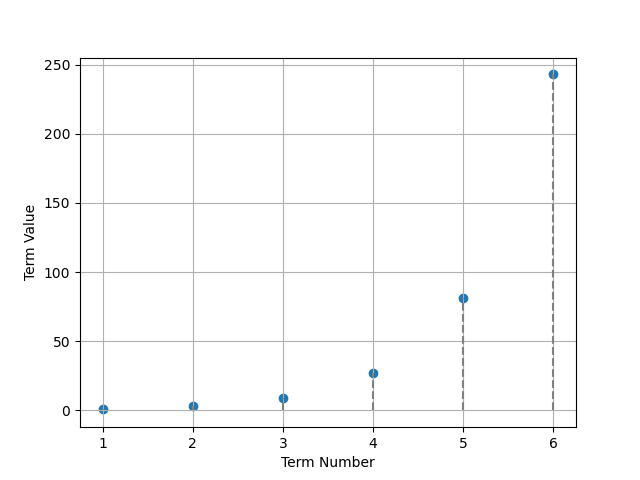
\includegraphics[width=1\columnwidth]{graph.png}
\label{fig:Graph1}
\end{figure}
\end{document}
